\scanpage{109}
\deleted{\unsure{soit|ait}} \inserted{l'on ait} $M(r)\leq e^{(r^\sigma)}$ pour $r$ assez grand.

\margin{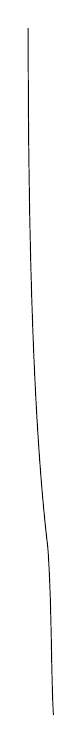
\begin{tikzpicture}[x=0.1mm,y=0.1mm,baseline=(current bounding box.north)]
\draw[line width=0.35pt] (0,0) .. controls (0,-260) and (6,-500) .. (25,-660) .. controls (30,-730) and (29,-815) .. (32,-872);
\end{tikzpicture}}
\uline{Théorème 2} (Hadamard-Borel) Si l'ordre $\rho$ de $f(z)$
est fini, alors pour \deleted{tout} $\varepsilon>0$, la série
\[
\sum{}'\frac{1}{|a_n|^{\rho+\varepsilon}}<+\infty \tag*{(5)}
\]
($'$ indique
qu'on ne somme pas sur les racines nulles)

De plus, on a alors (en supposant $f(0)\ne0$)
\[
f(z)=e^{P(z)}\prod_n\left(1-\frac{z}{a_n}\right)e^{\frac{z}{a_n}+\mathord{-}+\frac{z^p}{p a_n^p}}
\]
où $p\leq\rho$, et $P(z)$ est \deleted{\unsure{un polynôme}} \inserted{un polynôme}
de degré $\leq\rho$ : en d'autres termes, on
a \qquad genre de $f$ $\leq\rho=$ ordre de $f$

\uline{Corollaire} \quad Si $\rho<1$, i.e s'il existe un $0<\mu<1$
tel que $M(r)\leq e^{(r^\mu)}$ pour $r$ assez grand,
alors $f(z)$ est de genre zéro :
\[
f(z)=\mathrm{c}^{\mathrm{te}}\mathbin{\times}\prod_n\left(1-\frac{z}{a_n}\right)\deleted{\unsure{e^{z/a_n}}}
\]

\uline{Remarque}. \quad Il est très facile de se convaincre
que \qquad ordre de $f$ $\leq$ genre de $f+1$. Donc, si $\omega$ et
$g$ sont respectivement le genre et l'ordre, on a
\begin{center}
\makebox[0pt][l]{\raisebox{-2mm}{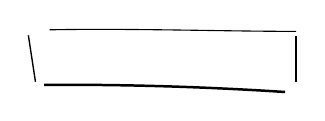
\begin{tikzpicture}[x=1mm,y=1mm]
\draw[line width=0.4pt] (2.7,7.2) .. controls (13,7.4) and (25,7.0) .. (34,7.0);
\draw[line width=0.5pt] (0,6.5) -- (0.9,0.6);
\draw[line width=0.45pt] (34,6.4) -- (34,0.6);
\draw[line width=0.9pt] (2,0.2) .. controls (14,0.3) and (25,-0.2) .. (32.6,-0.7);
\end{tikzpicture}}}\makebox[34mm]{\(\omega-1\leq g\leq\omega\)}
\end{center}

Comme $\gamma$ est entier, il en résulte que $\gamma$
est connu dès que $\omega$ l'est, sauf si $\omega$ est
entier. En ce cas, on peut avoir $p=\omega$, ou
$\gamma=\omega-1$
\margin{110}
